\documentclass[tikz,border=6pt]{standalone}

\usepackage{xcolor}
\usepackage{tikz}

% Colors
\definecolor{lightbluebg}{RGB}{238,244,255}
\definecolor{lightgreenbg}{RGB}{235,248,235}
\definecolor{varred}{RGB}{200,0,0}
\definecolor{magentaDef}{RGB}{180,0,120}
\definecolor{nameblue}{RGB}{40,90,160}
\definecolor{codegray}{RGB}{120,120,120}

\begin{document}

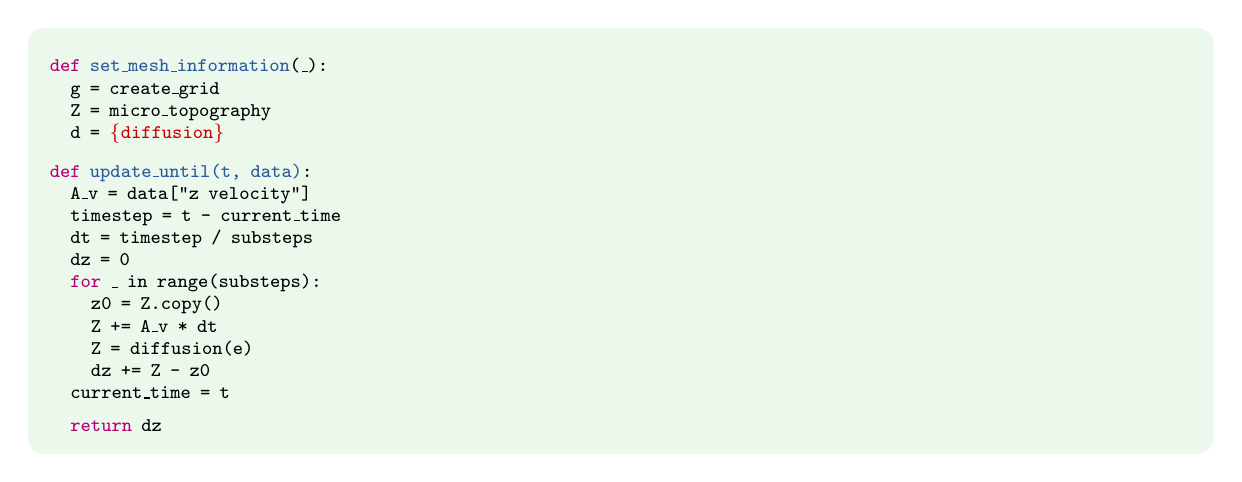
\begin{tikzpicture}

\node[
    fill=lightgreenbg,
    rounded corners=6pt,
    inner sep=8pt,
    text width=14.5cm
]{
\ttfamily\scriptsize

\textcolor{magentaDef}{def} \textcolor{nameblue}{set\_mesh\_information}(\_):\\
\quad g = create\_grid\\
% \quad \textcolor{codegray}{\# adds tiny irregularities (initial surface)}\\
\quad Z = micro\_topography\\
\quad d = \textcolor{varred}{\{diffusion\}}\\[6pt]

\textcolor{magentaDef}{def} \textcolor{nameblue}{update\_until(t, data)}:\\
\quad A\_v = data["z velocity"]\\

\quad timestep = t - current\_time\\
\quad dt = timestep / substeps\\

\quad dz = 0\\

\quad \textcolor{magentaDef}{for} \_ in range(substeps):\\
\qquad z0 = Z.copy()\\

\qquad Z += A\_v * dt\\
\qquad Z = diffusion(e)\\

\qquad dz += Z - z0\\

\quad current\_time = t\\
\quad \textcolor{magentaDef}{return} dz
};

\end{tikzpicture}

\end{document}